%
%
%   LQuiz 15 : 2022--03--31 (R)
%
%

\section{Exercise}

% Reference : OS C II.1.3E160

(4 pt) Let $f : [0,6] \rightarrow \reals$ be a piecewise constant function. A graph of $y = \displaystyle\int_{0}^{x} f(t) \spaceIntd \intd t$ is shown below.
\begin{center}
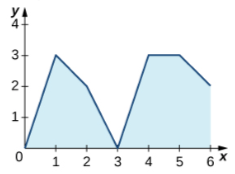
\includegraphics[scale=0.75]{\filePathGraphics/LQ15_Graph.png}
\end{center}

\begin{enumerate}[label=(\alph*)]
\item\label{itm : LQ15a} (2 pt) Over which intervals is $f$ positive? negative? equal to zero?
\end{enumerate}

\spaceSolution{1.5in}{% Begin solution.
View $y$ as a function of $x$, the cumulative signed area under the graph of $f$ from $t = 0$ to $t = x$. If $f$ is positive on some interval, then the signed area under the graph of $f$ is increasing on that interval. If $f$ is negative on some interval, then the signed area under the graph of $f$ is decreasing on that interval. If $f$ is zero on some interval, then the signed area under the graph of $f$ is not changing on that interval. The logical converse holds, too.

The fundamental theorem of calculus neatly captures this discussion, and more:
\begin{align}
y'
=
\frac{\intd}{\intd x} y
=
\frac{\intd}{\intd x} \int_{0}^{x} f(t) \spaceIntd \intd t
=
f(x)%
\label{eq : LQ15 FTC}
\end{align}
This equation says that the \emph{slope} of the cumulative signed area function $y$ at any point $x$ equals the \emph{value} of the function $f$ at $x$.

Analyzing the given graph, we see that $y' > 0$ on the interval $(0,1)$, so $f(x) = y' > 0$ on this interval. Similarly, $f(x) = y' < 0$ on the intervals $(1,2)$, $(2,3)$, and $(5,6)$; and $f(x) = y' = 0$ on the interval $(4,5)$.

\paragraph{Challenge:}

Why don't we include the endpoints of these intervals? Hint: Graph the cumulative signed area functions for the functions $f_{1} : [0,2] \rightarrow \reals$ and $f_{2} : [0,2] \rightarrow \reals$ given by
\begin{align*}
f_{1}(x)
&=
\begin{dcases*}
3	&	if $x \in [0,1]$	\\
-1	&	if $x \in (1,2]$
\end{dcases*}
&
f_{2}(x)
&=
\begin{dcases*}
3	&	if $x \in [0,1)$	\\
-1	&	if $x \in [1,2]$
\end{dcases*}
\end{align*}
What do you observe? Try to explain why this makes sense, in light of our theory.)}% End solution.



\begin{enumerate}[resume,label=(\alph*)]
\item\label{itm : LQ15b} (1 pt) What are the maximum and minimum values of $f$?
\end{enumerate}

\spaceSolution{1.5in}{% Begin solution.
Equation \eqref{eq : LQ15 FTC}, which we obtained by a straightforward application of the fundamental theorem of calculus, tells us that the value of $f(x)$ equals the slope of the cumulative signed area function $y$ at the input $x$. Thus the maximum (respectively, minimum) value of $f(x)$ equals the maximum (respectively, minimum) slope of $y$. From the graph, we see that the maximum value of $y'$, and hence of $f(x)$, is $3$ (take any point $x$ on the intervals $(0,1)$ or $(3,4)$); and the minimum value of $y'$, and hence of $f(x)$, is $-2$ (take any point $x$ on the interval $(2,3)$).}% End solution.



\pagebreak% Activate for solutions only!!!

\begin{enumerate}[resume,label=(\alph*)]
\item\label{itm : LQ15c} (1 pt) What is the average value of $f$ on the interval $[0,6]$?
\end{enumerate}

\spaceSolution{1.5in}{% Begin solution.
By definition, the average value of $f$ on the interval $[0,6]$ is
\begin{align*}
\frac{1}{6 - 0} \int_{0}^{6} f(x) \spaceIntd \intd x
\end{align*}
By definition of $y$, the value of $y$ at $x = 6$ is (the value of) the definite integral $\int_{0}^{6} f(x) \spaceIntd \intd x$. We can read this value off the graph of $y$, namely, $y(6) = 2$. Therefore the average value of $f$ on the interval $[0,6]$ is
\begin{align*}
\frac{1}{6} \int_{0}^{6} f(x) \spaceIntd \intd x
=
\frac{1}{6} (2)
=
\frac{1}{3}
\end{align*}

\paragraph{Challenge:}

We can say more! By definition, the average value of $f$ on the interval $[0,x]$ is
\begin{align*}
\frac{1}{x - 0} \int_{0}^{x} f(t) \spaceIntd \intd t
\end{align*}
This is the same definition we used above, except (i) we have replaced the right endpoint $6$ above with the variable $x$ here, because we analyzed the interval $[0,6]$ above, whereas here we analyze the interval $[0,x]$; and (ii) we use the variable of integration $t$ rather than $x$ here, because we're using $x$ as our upper endpoint on the integral.

I claim that if we compute this average value \emph{function}, we get
\begin{align*}
A(x)
=
\begin{dcases*}
3			&	if $x \in [0,1]$	\\
\frac{4}{x} - 1	&	if $x \in [1,2]$	\\
\frac{6}{x} - 2	&	if $x \in [2,3]$	\\
3 - \frac{9}{x}	&	if $x \in [3,4]$	\\
\frac{3}{x}		&	if $x \in [4,5]$	\\
\frac{8}{x} - 1	&	if $x \in [5,6]$
\end{dcases*}
\end{align*}
which is continuous. Can you validate this? Can you use the graph of $y$ above to check the values of this function, for example, on the integer values of $x$? How does our answer above, for the average value of $f$ on the interval $[0,6]$, fit into the framework of this average value function?}% End solution.